\documentclass[conference]{IEEEtran}
\usepackage{graphicx}
\usepackage{algorithm}
\usepackage{algorithmic}

\makeatletter
\def\BState{\State\hskip-\ALG@thistlm}
\makeatother



\begin{document}
\title{For a given value of n ($n > 3 $), generate an (n x n) matrix and scan the matrix with a (3 x 3) mask and find out those masks (mask positions) which are similar.}

\author{\IEEEauthorblockN{Parag Parihar}
\IEEEauthorblockA{Roll No:- IIT2016095\\
iit2016095@iiita.ac.in}
\and
\IEEEauthorblockN{Rakshit Sai}
\IEEEauthorblockA{Roll No:- IIT2016126\\
iit2016126@iiita.ac.in}
\and
\IEEEauthorblockN{Adarsh Agrawal}
\IEEEauthorblockA{Roll No:- IIT2016516\\
iit2016516@iiita.ac.in}
\and
\IEEEauthorblockN{Nilotpal Pramanik}
\IEEEauthorblockA{Roll No:- IRM2016501\\
irm2016501@iiita.ac.in}
\thanks{Manuscript received February 2, 2018.}}

\markboth{Assignment-1, IDAA432C; B.Tech.(IT)}
{Shell \MakeLowercase{\textit{et al.}}: Bare Demo of IEEEtran.cls for Journals}

\maketitle

\IEEEpeerreviewmaketitle

\section{\textbf{Introduction and Literature Survey}}
The give task for us was to design and analyse a problem.The problem given to us is to generate an (n x n) matrix whose cells are filled with randomly generated digits from 0 to 9. Then we have to take a matrix with a (3 x 3) mask from the given n x n matrix and find out those masks(mask positions) which are similar. For this purpose, we have to first define a similarity matrix to measure the similarity between two 3 x 3 matrices. We can also report the mask position by reporting a mask position by only mentioning top-left position of the mask.After finishing one cycle we have to go for the next mask.\\

Understanding the problem is very simple. It basically says that we need to keep on checking if each 3 x 3 matrix from the n x n matrix which we generate randomly is similar to the 3 x 3 mask which we will take from the original matrix and run over all the possible 3 x 3 matrices in the given n x n matrix. If we get a similar matrix then we note that matrix and represent the similar matrix with our own convention. Finally count the number of similar matrices and then analyze the code with proper graphs and examples. The line, you can represent the mask position by reporting a mask position by only mentioning top-left position of the mask states that, if we take a mask whose first number starts from A(i,j) of matrix A then we just represent the whole matrix by A(i,j) where i and j are particular indices of the top-left position of the 3 x 3 mask which we choose.   

\section{\textbf{Algorithm Design}}
\textbf{An algorithm For a given value of n ($n > 3 $), generate an (n x n) matrix and scan the matrix with a (3 x 3) mask and find out those masks (mask positions) which are similar:-}\\

According to the problem firstly we will scan $n$ to create a random matrix \textbf{\textit{matrix}} of $n * n$ and filled with digits  0 to 9 by using $srand(time(NULL))$.For any $n * n$ matrix the number of $3 * 3$ masks will be $(n-2)^2$.To store the unique masks we are creating an another matrix \textbf{\textit{store}} of size $(n-2) * (n-2)$ and initially that will be filled up with “-1”.\\

Now we will traverse the whole 2D array matrix \textbf{\textit{store}} and check if the index is equal to “-1” or not.If true then we will increment the value of \textbf{\textit{count\_of\_mask}},which indicates the number of distinct masks and has been initialized to 0 at the beginning.Otherwise we will proceed further by \textbf{continue}.We will also assign the value of \textbf{\textit{count\_of\_mask}} to the \textbf{\textit{store[i][j]}}.Now we have to traverse the input matrix \textbf{\textit{matrix}} through \textbf{\textit{k}} starting from the row index holder \textbf{\textit{i}} to $n-2$.If \textbf{\textit{k}} is equal to \textbf{\textit{i}} then we have start with the just next column i.e ${\textbf{\textit{j+1}}}_{th}$ instead of the corresponding ${\textbf{\textit{j}}}_{th}$ and the the value of column should be stored in \textbf{\textit{l}}.Otherwise we’ll assign 0 to \textbf{\textit{l}} and start traversing up to \textbf{\textit{n-2}} throughout the columns.Through out this procedure we are comparing the the other masks with a particular mask,chosen from the matrix.\\

There in \textbf{\textit{x}} we are receiving the return value of the \textbf{\textit{is\_similar}} function which is taking \textbf{\textit{i}},\textbf{\textit{j}},\textbf{\textit{k}},\textbf{\textit{l}} as the attributes to check whether two masks are similar or not.If similar it will return 1 and otherwise 0.If the \textbf{\textit{x}} is 1 the particular value of \textbf{\textit{count\_of\_mask}} will again assign to \textbf{\textit{store[k][l]}} and 0 will be assigned to \textbf{\textit{x}} again.\\

Now we will run for-loop from 1 to \textbf{\textit{count\_of\_mask}} through a variable.And by traversing the whole \textbf{\textit{store}} matrix we will check whether the particular position is equal to the value of that variable or not.If it is true then print the corresponding row and column indexes of that position.\\%After the end of the each iteration we will also check whether the value of \textbf{\textit{x}} is 1 or not.If it is true then we will proceed to the next line.\\


\begin{algorithm}[H]
\caption{issimilar function}
\end{algorithm}
\begin{algorithmic}[1]
\STATE \textbf{INPUT:-} i,j,k,l
\STATE \textbf{OUTPUT:-} True OR False
\FOR{$p=0 \ to \ 3$}
	\FOR{$q=0 \ to \ 3$}
    	\IF{matrix[i+p][j+q] != matrix[k+p][l+q]}
        	\STATE \textbf{return} $0$
         \ENDIF
      \ENDFOR
 \ENDFOR
 \STATE \textbf{return} $1$
\end{algorithmic}



\begin{algorithm}[H]
\caption{Generate $n*n$ matrix and scan the matrix with a (3 x 3) mask and find out those masks (mask positions) which are similar.}
\end{algorithm}
\begin{algorithmic}[1]
\STATE \textbf{INPUT: \textit{n}}
\STATE \textbf{OUTPUT: all similar mask positions.}
\STATE \textbf{Initialization} : $\textit{count\_of\_mask} \gets 0$
\STATE generate any random $ n*n $ matrix(\textit{matrix}) \textbf{filled with digits  0 to 9}
\STATE create a 2d matrix \textit{store[n-2][n-2]} filled with -1 
\FOR{$ i=0 \ to \ n-2$} 
	\FOR{$ j=0 \ to \ n-2$}
    	\IF{$store[i][j] != -1$}
        	 \STATE \textbf{continue}
        \ELSE
        	\STATE $count\_of\_mask \gets count\_of\_mask+1 $
        \ENDIF
       	\STATE $store[i][j] \gets count\_of\_mask$
        \FOR{$ k=0 \ to \ n-2$}
        	\IF{$k = i$}
            	\STATE $l \gets j+1$
            \ELSE 
            	\STATE $l \gets 0$
            \ENDIF
            \FOR{$l \ to \ n-2$}
            	\IF{$is\_similar(i,j,k,l)=1$}  
                	\STATE \textit{$store[k][l] \gets count\_of\_mask$}
                \ENDIF
            \ENDFOR
        \ENDFOR
    \ENDFOR
\ENDFOR
\FOR{$i=1 \ to \ count\_of\_mask$}
	\FOR{$j=0 \ to \ n-2$}
    	\FOR{$k=0 \ to \ n-2$}
        	\IF{$store[j][k] = i$}
            	\STATE print(j,k)
            \ENDIF
        \ENDFOR
   \ENDFOR
\ENDFOR
\end{algorithmic}



\section{\textbf{Analysis and Discussion}}
In our algorithm we have to generate a $n*n$ matrix but n should be greater than 3 ($ n>3 $).And we have to scan each mask and have to compare it with other masks. Our comparing(is\_similar) function will take constant time. 
\subsection{For Algorithm:-1}
This function is being used for comparing two $3*3$ mask. So in this case we need total 125 units of time.
\\ $$time_{for\_function}  = 125$$
\subsection{For Algorithm:- 2}
\subsubsection{\textbf{BEST CASE-}}
In this case all the elements in our $n*n$ matrix will be same and we will have to compare first mask to all the other mask only. We will not have to compare next mask to any other mask as because all the other mask will be already similar to the first mask.
\\\\\ $$time_{best\_case} \propto 140n^2-548n+541$$
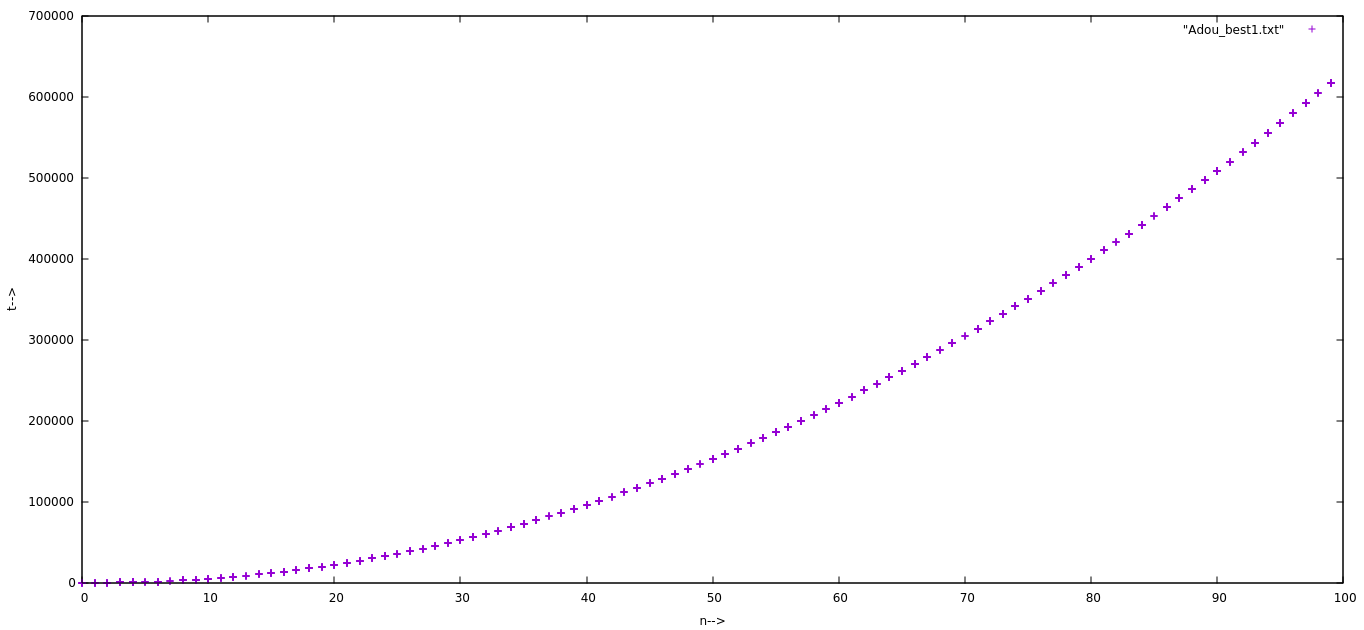
\includegraphics[height =  6.00cm,width = \linewidth]{best.png}
\subsubsection{\textbf{WORST CASE-}}
In this case all the elements in our matrix will be between 0 to 9. And there will not be any mask which will be similar to any other mask i.e. all the mask will be unique. So we will have to compare every mask to all other mask. 
\\$$time_{worst\_case} \propto 133n^4 -1057n^3 +3163n^2 - 4219n +2115$$
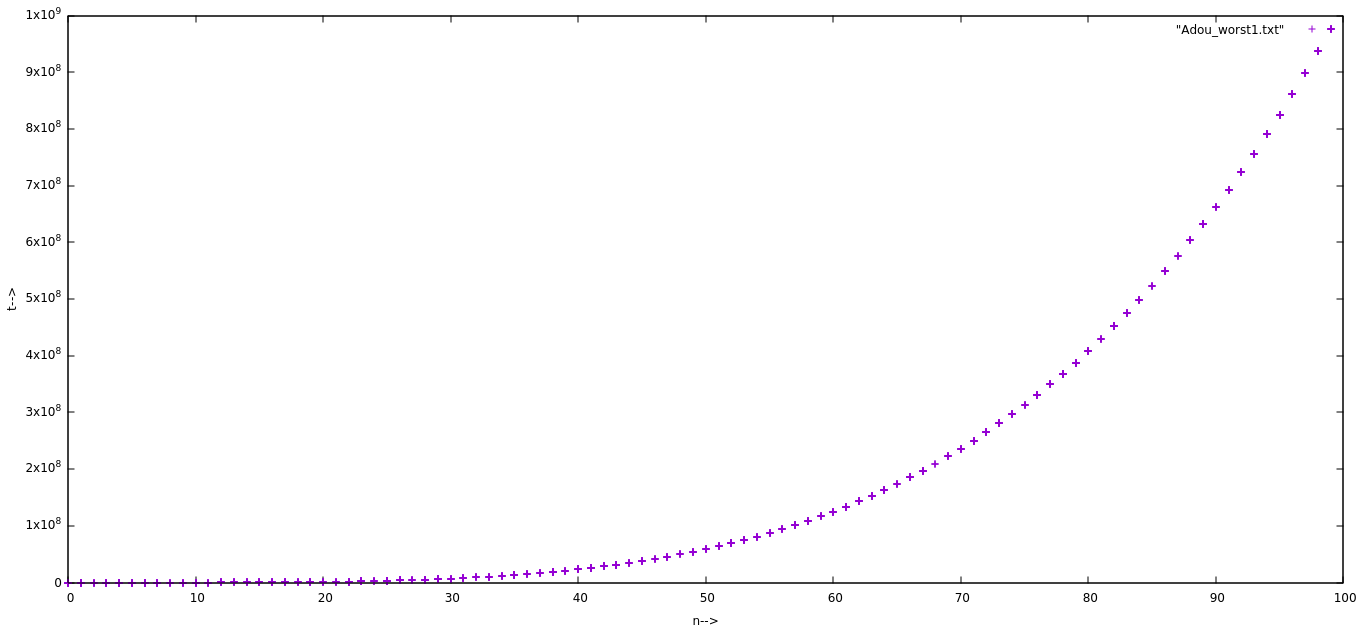
\includegraphics[height =  6.00cm,width = \linewidth]{worst.png}
\subsubsection{\textbf{AVERAGE CASE-}}
In this case we can not particularly say anything about time complexity of our $n*n$ matrix. As our matrix may have some similar mask.
\\ $$time_{best\_case} \leq time_{average\_case} \leq time_{worst\_case}$$
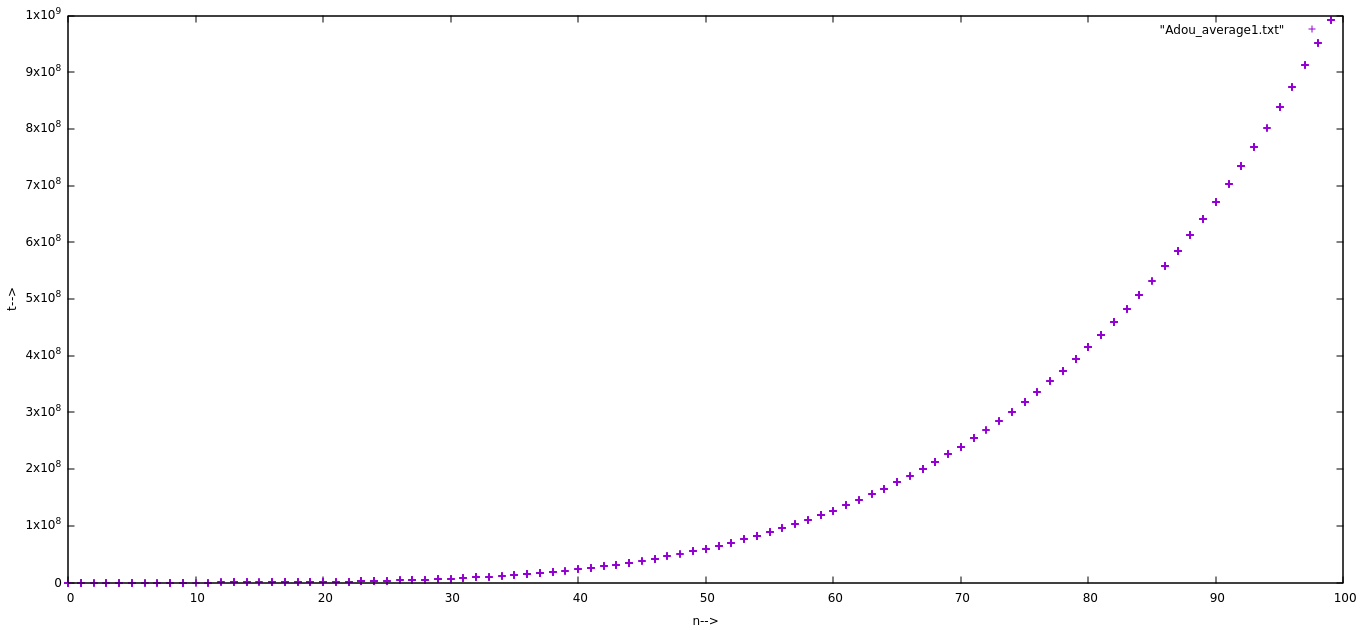
\includegraphics[height =  6.00cm,width = \linewidth]{average.png}
\section{\textbf{Experimental Study}}
We revised the commands and basic functions of \textbf{GNUPlot}
to plot the time complexity analysis graphs and other relevant
analysis related to our algorithm.
\\
\	While making this report we also learnt the basics of
making reports using LATEX in IEEE format using \textbf{IEEEtran
class}.
\\\\
For the analysis of the Complexity of the algorithm we had to generate 3 kinds of testcases. For each of these 3 kinds our code was run on \textbf{1000} testcases of each type and The algorithm was run on these three files separately and graphs were plotted using \textbf{GNU-Plot}.The graphs have been vividly explained in the previous section. In each of these testcases the size of \textbf{row} and \textbf{coloumn}(row and coloumn are equal) was randomly chosen greater then 3.
\\
\\
For the \textbf{Best case}, we generated the testases where matrix was filled with same number(random generated between 0 to 9).
\\
\begin{table}[h!]
\begin{center}
    \label{tab:table1}
    \begin{tabular}{|c|c|c|c|} % <-- Alignments: 1st column left, 2nd middle and 3rd right, with vertical lines in between
    \hline
      \textbf{n} & $\textbf{{time}}_{{best case}}$ & $\textbf{{time}}_{{average case}}$ & $\textbf{{time}}_{{worst case}}$
      \\
      \hline
      5 & 764 & 1310 & 1329\\
      \hline
      10 & 4614 & 48000 & 48686\\
      \hline
      20 & 22064 & 1178036 & 1195682\\
      \hline
      50 & 152414 & 58761320 & 59659358\\
      \hline
	  75 & 350414 & 313631270 & 318423415\\
      \hline
	  100 & 629664 & 1017577470 & 1033132346\\
      \hline
    \end{tabular}
\end{center}
\end{table}
\\
For the \textbf{Worst case},we generated testcases where matrix was filled with numbers uniquely to avoid any similar mask throughout the 2d matrix.\\
\\
 And for the \textbf{average case},we generated testcases where matrix was filled with numbers between 0 to 9 so that there may be some similar masks.
 \\
\section{\textbf{Conclusion}}
According the problem we have to write an algorithm For a given value of n ($n > 3 $), generate an (n x n) matrix and scan the matrix with a (3 x 3) mask and find out those masks (mask positions) which are similar.Through different experimental studies we have tried to analyze this algorithm perfectly and properly.\\

In worst case we got the time complexity $O(n^4)$ where as in best case we were able to reduce the time complexity to $\Omega(n^2)$.But the average case is not too clear as we are taking the randomly generated matrix as the input matrix.But by taking different samples of input and analyzing the corresponding output we can conclude that the time complexity is lying in between the worst and best case time complexity.


\end{document}
